\chapter{Scenario}
\label{chap-scenario-1}

\begin{figure}[H]
\centering
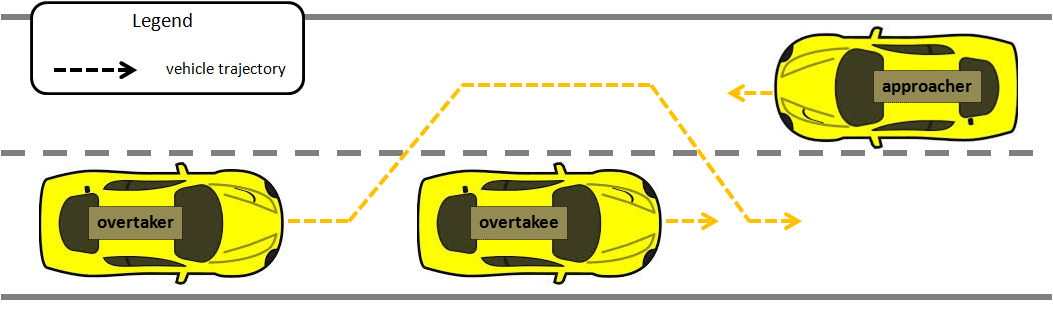
\includegraphics[width=\textwidth]{figures/overtakingWithApproacher.png}
\caption{Scenario}
\label{fig:scenario}
\end{figure}

In this scenario, there are three vehicles driving in two-lane road. Figure \ref{fig:scenario} shows the road and the three vehicles. Two vehicles drive one after another in one direction, while the third vehicle drives on the other lane in the opposite direction. The first two vehicles are named \textit{Overtaker} and \textit{Overtakee}. The third vehicle is named \textit{Approacher}. 

The \textit{Overtaker} wants to overtake the \textit{Overtakee} in a safe manner. This means that the \textit{Approacher} should be far enough during the overtaking. Otherwise, the overtaking should not be allowed. The vehicles can exchange messages in order to assure the safety in this scenario.  

  